% Created by tikzDevice version 0.12.6 on 2026-09-22 18:56:48
% !TEX encoding = UTF-8 Unicode
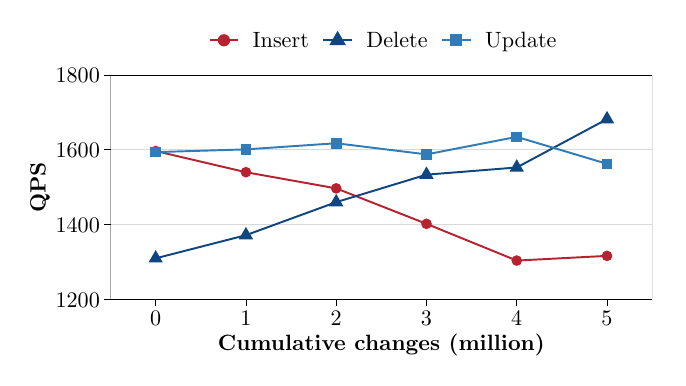
\begin{tikzpicture}[x=1pt,y=1pt]
\definecolor{fillColor}{RGB}{255,255,255}
\path[use as bounding box,fill=fillColor,fill opacity=0.00] (0,0) rectangle (227.65,119.25);
\begin{scope}
\path[clip] (  0.00,  0.00) rectangle (227.65,119.25);
\definecolor{fillColor}{RGB}{255,255,255}

\path[fill=fillColor] (  0.00,  0.00) rectangle (227.65,119.25);
\end{scope}
\begin{scope}
\path[clip] ( 29.95, 21.02) rectangle (225.65,102.13);
\definecolor{fillColor}{RGB}{255,255,255}

\path[fill=fillColor] ( 29.95, 21.02) rectangle (225.65,102.13);
\definecolor{drawColor}{gray}{0.85}

\path[draw=drawColor,line width= 0.3pt,line join=round] ( 29.95, 21.02) --
	(225.65, 21.02);

\path[draw=drawColor,line width= 0.3pt,line join=round] ( 29.95, 48.06) --
	(225.65, 48.06);

\path[draw=drawColor,line width= 0.3pt,line join=round] ( 29.95, 75.09) --
	(225.65, 75.09);

\path[draw=drawColor,line width= 0.3pt,line join=round] ( 29.95,102.13) --
	(225.65,102.13);
\definecolor{drawColor}{RGB}{183,34,48}

\path[draw=drawColor,line width= 0.7pt,line join=round] ( 46.26, 74.67) --
	( 78.87, 67.02) --
	(111.49, 61.18) --
	(144.11, 48.37) --
	(176.72, 35.09) --
	(209.34, 36.79);
\definecolor{drawColor}{RGB}{16,70,128}

\path[draw=drawColor,line width= 0.7pt,line join=round] ( 46.26, 35.90) --
	( 78.87, 44.27) --
	(111.49, 56.20) --
	(144.11, 66.13) --
	(176.72, 68.73) --
	(209.34, 86.19);
\definecolor{drawColor}{RGB}{49,124,183}

\path[draw=drawColor,line width= 0.7pt,line join=round] ( 46.26, 74.28) --
	( 78.87, 75.27) --
	(111.49, 77.49) --
	(144.11, 73.46) --
	(176.72, 79.79) --
	(209.34, 70.05);
\definecolor{fillColor}{RGB}{183,34,48}

\path[fill=fillColor] ( 46.26, 74.67) circle (  1.93);

\path[fill=fillColor] ( 78.87, 67.02) circle (  1.93);

\path[fill=fillColor] (111.49, 61.18) circle (  1.93);

\path[fill=fillColor] (144.11, 48.37) circle (  1.93);

\path[fill=fillColor] (176.72, 35.09) circle (  1.93);

\path[fill=fillColor] (209.34, 36.79) circle (  1.93);
\definecolor{fillColor}{RGB}{16,70,128}

\path[fill=fillColor] ( 46.26, 38.90) --
	( 48.85, 34.40) --
	( 43.66, 34.40) --
	cycle;

\path[fill=fillColor] ( 78.87, 47.26) --
	( 81.47, 42.77) --
	( 76.28, 42.77) --
	cycle;

\path[fill=fillColor] (111.49, 59.20) --
	(114.09, 54.71) --
	(108.89, 54.71) --
	cycle;

\path[fill=fillColor] (144.11, 69.13) --
	(146.70, 64.63) --
	(141.51, 64.63) --
	cycle;

\path[fill=fillColor] (176.72, 71.73) --
	(179.32, 67.23) --
	(174.13, 67.23) --
	cycle;

\path[fill=fillColor] (209.34, 89.19) --
	(211.94, 84.69) --
	(206.75, 84.69) --
	cycle;
\definecolor{fillColor}{RGB}{49,124,183}

\path[fill=fillColor] ( 44.33, 72.35) --
	( 48.18, 72.35) --
	( 48.18, 76.21) --
	( 44.33, 76.21) --
	cycle;

\path[fill=fillColor] ( 76.95, 73.34) --
	( 80.80, 73.34) --
	( 80.80, 77.20) --
	( 76.95, 77.20) --
	cycle;

\path[fill=fillColor] (109.56, 75.56) --
	(113.42, 75.56) --
	(113.42, 79.42) --
	(109.56, 79.42) --
	cycle;

\path[fill=fillColor] (142.18, 71.53) --
	(146.04, 71.53) --
	(146.04, 75.38) --
	(142.18, 75.38) --
	cycle;

\path[fill=fillColor] (174.80, 77.86) --
	(178.65, 77.86) --
	(178.65, 81.72) --
	(174.80, 81.72) --
	cycle;

\path[fill=fillColor] (207.41, 68.12) --
	(211.27, 68.12) --
	(211.27, 71.97) --
	(207.41, 71.97) --
	cycle;
\definecolor{drawColor}{RGB}{0,0,0}

\path[draw=drawColor,line width= 0.4pt,line join=round,line cap=round] ( 29.95, 21.02) rectangle (225.65,102.13);
\end{scope}
\begin{scope}
\path[clip] (  0.00,  0.00) rectangle (227.65,119.25);
\definecolor{drawColor}{RGB}{0,0,0}

\node[text=drawColor,anchor=base east,inner sep=0pt, outer sep=0pt, scale=  0.80] at ( 26.07, 18.26) {1200};

\node[text=drawColor,anchor=base east,inner sep=0pt, outer sep=0pt, scale=  0.80] at ( 26.07, 45.30) {1400};

\node[text=drawColor,anchor=base east,inner sep=0pt, outer sep=0pt, scale=  0.80] at ( 26.07, 72.34) {1600};

\node[text=drawColor,anchor=base east,inner sep=0pt, outer sep=0pt, scale=  0.80] at ( 26.07, 99.38) {1800};
\end{scope}
\begin{scope}
\path[clip] (  0.00,  0.00) rectangle (227.65,119.25);
\definecolor{drawColor}{RGB}{0,0,0}

\path[draw=drawColor,line width= 0.3pt,line join=round] ( 27.67, 21.02) --
	( 29.95, 21.02);

\path[draw=drawColor,line width= 0.3pt,line join=round] ( 27.67, 48.06) --
	( 29.95, 48.06);

\path[draw=drawColor,line width= 0.3pt,line join=round] ( 27.67, 75.09) --
	( 29.95, 75.09);

\path[draw=drawColor,line width= 0.3pt,line join=round] ( 27.67,102.13) --
	( 29.95,102.13);
\end{scope}
\begin{scope}
\path[clip] (  0.00,  0.00) rectangle (227.65,119.25);
\definecolor{drawColor}{RGB}{0,0,0}

\path[draw=drawColor,line width= 0.3pt,line join=round] ( 46.26, 18.74) --
	( 46.26, 21.02);

\path[draw=drawColor,line width= 0.3pt,line join=round] ( 78.87, 18.74) --
	( 78.87, 21.02);

\path[draw=drawColor,line width= 0.3pt,line join=round] (111.49, 18.74) --
	(111.49, 21.02);

\path[draw=drawColor,line width= 0.3pt,line join=round] (144.11, 18.74) --
	(144.11, 21.02);

\path[draw=drawColor,line width= 0.3pt,line join=round] (176.72, 18.74) --
	(176.72, 21.02);

\path[draw=drawColor,line width= 0.3pt,line join=round] (209.34, 18.74) --
	(209.34, 21.02);
\end{scope}
\begin{scope}
\path[clip] (  0.00,  0.00) rectangle (227.65,119.25);
\definecolor{drawColor}{RGB}{0,0,0}

\node[text=drawColor,anchor=base,inner sep=0pt, outer sep=0pt, scale=  0.80] at ( 46.26, 11.63) {0};

\node[text=drawColor,anchor=base,inner sep=0pt, outer sep=0pt, scale=  0.80] at ( 78.87, 11.63) {1};

\node[text=drawColor,anchor=base,inner sep=0pt, outer sep=0pt, scale=  0.80] at (111.49, 11.63) {2};

\node[text=drawColor,anchor=base,inner sep=0pt, outer sep=0pt, scale=  0.80] at (144.11, 11.63) {3};

\node[text=drawColor,anchor=base,inner sep=0pt, outer sep=0pt, scale=  0.80] at (176.72, 11.63) {4};

\node[text=drawColor,anchor=base,inner sep=0pt, outer sep=0pt, scale=  0.80] at (209.34, 11.63) {5};
\end{scope}
\begin{scope}
\path[clip] (  0.00,  0.00) rectangle (227.65,119.25);
\definecolor{drawColor}{RGB}{0,0,0}

\node[text=drawColor,anchor=base,inner sep=0pt, outer sep=0pt, scale=  0.80] at (127.80,  2.56) {\bfseries Cumulative changes (million)};
\end{scope}
\begin{scope}
\path[clip] (  0.00,  0.00) rectangle (227.65,119.25);
\definecolor{drawColor}{RGB}{0,0,0}

\node[text=drawColor,rotate= 90.00,anchor=base,inner sep=0pt, outer sep=0pt, scale=  0.80] at (  6.52, 61.57) {\bfseries QPS};
\end{scope}
\begin{scope}
\path[clip] (  0.00,  0.00) rectangle (227.65,119.25);
\definecolor{fillColor}{RGB}{255,255,255}

\path[fill=fillColor] ( 64.51,110.13) rectangle (191.09,118.25);
\end{scope}
\begin{scope}
\path[clip] (  0.00,  0.00) rectangle (227.65,119.25);
\definecolor{drawColor}{RGB}{183,34,48}

\path[draw=drawColor,line width= 0.7pt,line join=round] ( 65.79,114.69) -- ( 76.04,114.69);
\definecolor{fillColor}{RGB}{183,34,48}

\path[fill=fillColor] ( 70.92,114.69) circle (  2.21);
\end{scope}
\begin{scope}
\path[clip] (  0.00,  0.00) rectangle (227.65,119.25);
\definecolor{drawColor}{RGB}{16,70,128}

\path[draw=drawColor,line width= 0.7pt,line join=round] (106.88,114.69) -- (117.12,114.69);
\definecolor{fillColor}{RGB}{16,70,128}

\path[fill=fillColor] (112.00,118.13) --
	(114.98,112.97) --
	(109.02,112.97) --
	cycle;
\end{scope}
\begin{scope}
\path[clip] (  0.00,  0.00) rectangle (227.65,119.25);
\definecolor{drawColor}{RGB}{49,124,183}

\path[draw=drawColor,line width= 0.7pt,line join=round] (149.79,114.69) -- (160.03,114.69);
\definecolor{fillColor}{RGB}{49,124,183}

\path[fill=fillColor] (152.70,112.48) --
	(157.12,112.48) --
	(157.12,116.90) --
	(152.70,116.90) --
	cycle;
\end{scope}
\begin{scope}
\path[clip] (  0.00,  0.00) rectangle (227.65,119.25);
\definecolor{drawColor}{RGB}{0,0,0}

\node[text=drawColor,anchor=base west,inner sep=0pt, outer sep=0pt, scale=  0.80] at ( 81.32,111.93) {Insert};
\end{scope}
\begin{scope}
\path[clip] (  0.00,  0.00) rectangle (227.65,119.25);
\definecolor{drawColor}{RGB}{0,0,0}

\node[text=drawColor,anchor=base west,inner sep=0pt, outer sep=0pt, scale=  0.80] at (122.40,111.93) {Delete};
\end{scope}
\begin{scope}
\path[clip] (  0.00,  0.00) rectangle (227.65,119.25);
\definecolor{drawColor}{RGB}{0,0,0}

\node[text=drawColor,anchor=base west,inner sep=0pt, outer sep=0pt, scale=  0.80] at (165.31,111.93) {Update};
\end{scope}
\end{tikzpicture}
